\chapter{The Research Project}\label{C:aim}

In this chapter, we outline the main ideas and objectives of this research project. 
%%% ACF Only complexity?
Section One discusses complexity analysis in time series, highlighting its advantages and limitations. 
%%% ACF Use numbered sections/subsections and refer to their automatic numbers
Section~\ref{Sec:AdvantagesLimitations} examines the limitations of the Bandt and Pompe method. 
Section Three provides background knowledge on the 
%%% ACF What is this plane?
statistical complexity plane. 
Section Four explores the entropy-complexity plane for a broad class of time series. Section five provides the asymptotic distribution of the entropy. Finally, the chapter concludes with the objectives of the research project and a case study related to our work.

%%% ACF Do you analyse complexity only?
\section{Complexity Analysis in Time Series: Advantages and Limitations}\label{Sec:AdvantagesLimitations}

While this method effectively captures ordinal relationships between data points, it has notable drawbacks. 
First, it ignores amplitude information in the time series. 
%%% ACF "complexity-entropy plane"?
Second, classifying data via the complexity-entropy plane becomes challenging (or even misleading) in high-dimensional chaotic systems, 
%%% ACF Do you know what chaotic systems are?
%%% ACF Read and study about the logistic map
%%% ACF What is surrogate data?
as both deterministic chaotic time series and stochastic surrogate data may occupy overlapping regions within the plane.

%%% ACF I think that when you refer to "statistical complexity measures" you are referring to "information theory-based measures"
Despite these limitations, integrating statistical complexity measures such as those derived from the complexity-entropy plane offers a robust framework to enhance ordinal pattern analysis. 
%%% ACF Not only from the (marginal) distribution, but also from the independence
%%% ACF What a dynamical proces is?
These measures quantify deviations from uniform ordinal pattern distributions, enabling a more nuanced characterization of dynamical processes. 
%%% ACF Cite your sources, otherwise the text is yours
By combining permutation entropy with statistical complexity, researchers gain a refined tool to differentiate stochastic signals from deterministic chaos, thereby revealing intricate structural patterns and degrees of randomness in time series data.

\section{The Bandt and Pompe Method: A Robust Approach}

%%% ACF Reserve "demonstrate" for mathetical proofs
The concept of ordinal patterns in time series can be effectively demonstrated through real world examples. 
Traditionally, numerous algorithms, techniques, and heuristics have been employed to estimate complexity measures from real world data. 
%%% ACF What is a low-dimensional dynamical system?
However, these methods often perform well only for low dimensional dynamical systems and struggle when noise is introduced.

%%% ACF What is the Lyapunov exponent?
The Bandt and Pompe method overcomes this limitation by providing a robust approach that remains reliable even in noisy environments. 
In time series analysis, key complexity measures such as entropy, fractal dimension, and Lyapunov exponents play a crucial role in comparing neighboring values and uncovering the underlying structure and dynamics of the data.

The advantages of Bandt \& Pompe methods:
\begin{itemize}
	\item Simplicity
	\item Extremely fast calculation
	\item Robutness
	\item Invariance to nonlinear monotonous transformations
\end{itemize}	

This method exhibits low sensitivity to noise and naturally accounts for the causal order of elements in a time series. As a result, it can be applied to various real-world problems, particularly in differentiating between chaotic and stochastic signals.

Despite its limitations, researchers have developed extensions to the original method to address its shortcomings and enhance its applicability to a broader range of complex systems.

\section{Statistical Complexity measures}

After Bandt and Pompe introduced a successful method for analyzing time series, Rosso et al.~\cite{Rosso2007} expanded on this approach by incorporating the  statistical complexity derived from the same histogram of causal patterns. 
This method, which utilizes the complexity-entropy plane, has been successfully applied to various dynamic regimes including, 
%%% ACF What is system parameter change?
system parameter change
%%% ACF Sort the citation number
%%% ACF You must have an idea of every paper you cite
\cite{Cao2004,Bandt2005,Kowalski2007,Zunino2010a,Rosso2010a,Kowalski2011b,Zunino2012a, DeMicco2012a}, 
%%% ACF What is optical chaos
optical chaos \cite{Soriano2011a,Zunino2011a,Toomey2014,Yang2015e,Liu2016f}, hydrology \cite{Lange2013,Serinaldi2014,Stosic2016}, geophysics \cite{Consolini2014,Saco2010,Sippel2016}, engineering \cite{Yan2012,Aquino2015,Aquino2017,Redelico2017a}, biometrics \cite{Rosso2016}, characterization of pseudo-random number generators \cite{DeMicco2008,DeMicco2009}, biomedical signal analysis \cite{Zanin2012,Li2007,Li2008b,Parlitz2012,Morabito2012,Li2014b,Montani2014,Montani2014a,Liang2015b,Montani2015a,Montani2015}, econophysics \cite{Zanin2012,Zunino2010,Zunino2009, Bariviera2015a,Bariviera2015,Bariviera2016,Zunino2016a}.

After computing all symbols as described in Chapter~\ref{C:intro}, the histogram proportions are used to estimate the probability distribution of ordinal patterns. 
From this distribution, two key descriptors are calculated to characterize the time series:
\begin{enumerate}
\item Entropy (a measure of system disorder)

\item Statistical complexity
\end{enumerate}
The most common metric for the first descriptor is the normalized Shannon entropy, defined as:
\begin{equation}
	H(\mathbf{p})=-\dfrac{1}{\log k}\sum^{k}_{j=1}p_j \ln{p_j}.
\end{equation}
Here, $k=D!$ represents the total number of possible permutation patterns, and
%%% ACF Something is missing here
 terms in the summation where $p_j$ are excluded by convention. This entropy is bounded within the unit interval:
\begin{itemize}
\item It reaches its minimum value $(H=0)$ when a single pattern dominates  for some $p_j=1$ for some $j$ 
\item It achieves its maximum $(H=1)$ under uniform probability $p_j=1/k$ for all $j$ for all. 
\end{itemize}
This normalized entropy is often termed permutation entropy in time series analysis. 

While normalized Shannon entropy is a powerful tool for quantifying disorder, it fails to fully characterize complex dynamics. To address this limitation, López-Ruiz et al.~\cite{lopez1995statistical} introduced the disequilibrium $Q$ concept, which quantifies the deviation of a probability distribution $\mathbf{p}$ from a uniform (non-informative) equilibrium state. 
%%% ACF Here you say that the disequilibrium is the Euclidean distance, but then you say that it is the Jensen-Shannon
Specifically, disequilibrium measures the Euclidean distance between $\mathbf{p}$ and the uniform distribution, providing a complementary metric to Shannon entropy for assessing structural complexity in systems.

The Jensen-Shannon distance ($Q'$) between histogram of proportion $\mathbf{p}$ and the uniform probability function $\mathbf{u}=u_1,u_2,\dots, u_k$, where $k=D!$ corresponds to the number of possible permutation patterns—provides a robust metric for quantifying deviations from uniformity. This distance measure, derived from the symmetric Jensen-Shannon divergence, is particularly suited for analyzing ordinal pattern distributions due to its ability to capture both structural differences and statistical equilibrium in time series data.
Here is the formula for $Q'$:
\begin{equation}
	Q'(\mathbf{p,u})=\sum^k_{\ell=1} p_\ell\log\dfrac{p_\ell}{u_\ell}+u_\ell\log\dfrac{u_\ell}{p_\ell}
\end{equation}

Lamberti et al. \cite{lamberti2004intensive} proposed Jensen-Shannon distance as a symmetric metric rooted in the Jensen-Shannon divergence. As the reference model, most works consider the uniform distribution $\mathbf{u}=(1/k,1/k, \dots, 1/k)$. The normalized disequilibrium is defined as follows
\begin{equation}
	Q=\dfrac{Q'}{\max{(Q')}},
\end{equation}
where $\max(Q')$ is defined as follows
\begin{equation}
	\max(Q')=-2 \left[\dfrac{k+1}{k}\log(k+1)-2\log(2k)+\log k\right].
\end{equation}

After this concept, Lamberti et al. \cite{lamberti2004intensive} proposed \textbf{Statistical Complexity Measure} which is defined as 
\begin{equation}
	C=HQ
\end{equation}
where both $H$ and $Q$ are normalized quantities, therefore $C$ is also normalized. 
  
\section{The Entropy Complexity Plane}
The complexity-entropy plane is a two-dimensional representation where time series are mapped based on their permutation entropy and statistical complexity. These metrics are derived from ordinal pattern distributions obtained through time-delay embedding—a technique involving:
\begin{itemize}
	\item Embedding dimension $D$: Determines the number of permutation patterns $D!$ used to construct histograms.
	\item Time delay $(\tau)$: Often optimized for specific applications 
\end{itemize} 


\subsection{Key Dynamics in the plane}
\begin{enumerate}
	\item Highly Ordered Systems
	
	Example: Strictly monotonic time series.
	\begin{itemize}
		\item Produces a single ordinal pattern $(H=0)$.
		
		\item Maximal disequilibrium (distance from uniform distribution).
		
		\item Maps to $(0,0),$ indicating minimal complexity.
	\end{itemize}
	
	\item Perfectly Random Systems
	
	Example: White noise
	\begin{itemize}
		\item Uniform ordinal pattern distribution $(H=1)$.
		\item Disequilibrium vanishes (distance $=0)$.
		\item Maps to $(1,0),$ reflecting maximal entropy without structural complexity.
	\end{itemize}
\end{enumerate}
The two extreme values are proved by Anteneodo \& Plastino \cite{anteneodo1996some}.Expressions for the boundaries, derived using geometrical arguments within space configurations, were proposed by Martin et al. \cite{Martin2006}. These formulations provide a structured approach to understanding and analyzing the spatial behavior of specific systems or models. The lower boundary is characterized by a smooth curve, whereas the upper boundary consists of $D!-1$ distinct segments. As the embedding dimension $D$ approaches infinity, the upper boundary gradually converges into a smooth curve. 
Example for the entropy complexity plane is shown in Figure \ref{fig:complexity}

\begin{figure}[H]
	\centering
	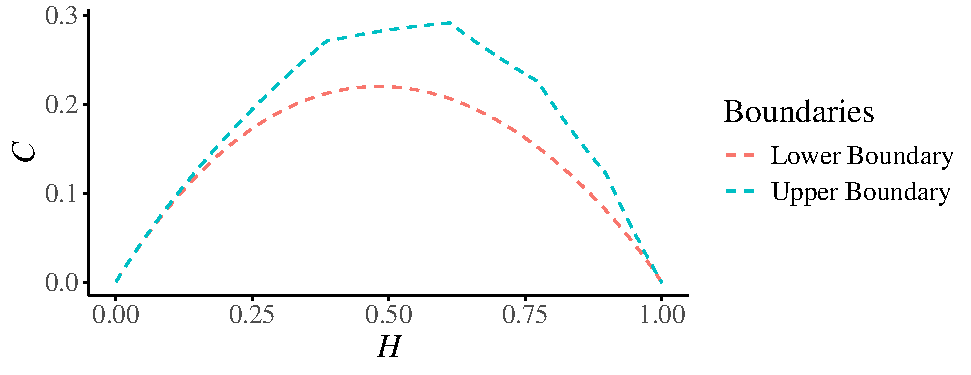
\includegraphics[width=0.6\textwidth]{complexity plane}
	\caption{Entropy Complexity Plane for Embedding dimension 3}
	\label{fig:complexity}
\end{figure}

\section {Asymptotic Distribution of the Shannon Entropy under the Multinomial Distribution}

The Multinomial distribution describes how observations fall into categories when an adequate model is available. It is similar to the multivariate normal distribution, which is one of the continuous Multivariate distributions. Furthermore, it has received considerable attention from researchers, both in theoretical studies and in applications related to discrete multivariate distributions. 
The normalized Shannon entropy, often employed in applications like permutation entropy, can be rigorously connected to its asymptotic distribution through the lens of statistical estimation theory. When estimating entropy from finite data, the plug-in estimator (computed directly from observed frequencies) converges to a normal distribution as the sample size $N\longrightarrow \infty$ even for dependent processes such as Markov chains. 
%%This asymptotic normality, demonstrated by Martin et al~\cite{M} 
%%% ACF Check the correct author/reference above
%%and Chagas et al~\cite{Chagas2022}, ensures that the estimator’s fluctuations around the true entropy value are Gaussian-distributed, with variance and bias determined by the underlying system’s dynamics. 
The Statistical properties of entropy measures under Multinomial distributions are crucial for analyzing complex systems where entropy serves as a key descriptors. Rey at al~\cite{Rey2023} investigate the asymptotic distributions of various entropy measures specifically, the Rényi and Tsallis entropies of order $q$, as well as Fisher information when these are computed using maximum likelihood estimators of probabilities from Multinomial random samples. The authors demonstrate that the Tsallis entropy and Fisher information asymptotically follow a normal distribution, whereas the Rényi entropy does not exhibit asymptotic normality. Through simulation studies, the paper validates that these asymptotic models effectively describe a variety of data scenarios. Additionally, the study introduces test statistics for comparing different types of entropies derived from two samples, even when the samples have differing numbers of categories. An application of these tests to social survey data indicates that the results are consistent and offer a more general approach compared to traditional chi-squared tests. 

 
In a subsequent study, Rey et al \cite{Rey2025} focus on the statistical complexity measure defined as the product of normalized Shannon entropy and the Normalized Jensen-Shannon divergence between a given probability distribution and the uniform distribution. 
They derive the asymptotic distribution of this complexity measure under the assumption that the observed data follow a Multinomial distribution. Further the study demonstrates that, as the sample size increases, the distribution of the statistical complexity converges to a normal distribution, with its variance and bias determined by the dynamics of the underlying system. This result provides a theoretical foundation for using statistical complexity as a tool for analyzing systems where the probability distributions are estimated from finite samples. The results are validated with theoretical findings through numerical experiments, showing that the asymptotic normality holds even in scenarios where the Multinomial model is not strictly applicable, such as in applications involving Bandt and Pompe ordinal patterns. 

Crucially, the convergence rate and limiting distribution depend on the system’s correlation structure deviating from the Multinomial case but remain tractable via spectral analysis of the transition matrix or ordinal pattern distributions \cite{PhysRevE.103.022215,Chagas2022}. This connection underscores the reliability of normalized entropy measures in large data regimes while highlighting the need to account for dependence structures in finite sample applications.


Imagine a sequence of $n$ independent trials, each resulting in precisely one outcome from a set of $k$ distinct possibilities labeled $\pi^1,\pi^2, \dots, \pi^k$ and so on. These outcomes are mutually exclusive, meaning only one can occur per trial, with respective probabilities $\bm{p}={\left\{p_1,p_2,\dots,p_k\right\}}$, such that $p_\ell \geq 0$ and $\sum^{k}_{\ell=1} {p_\ell =1}.$ The random vector $\bm{N}=(N_1,N_2,\dots, N_k)$ counts the number of occurrences of the events $\pi^1,\pi^2, \dots, \pi^k$ in the $n$ trials, with $N_\ell \geq0$ and $\sum^{k}_{\ell=1} {N_\ell =n}.$ A $\bm{n}$ is a sample from $\bm{N}$ and it has a $k-$variate vector of integer values $\bm{n}=(n_1,n_2,\dots,n_k).$ Then the joint distribution of $\bm{N}$ is 
\begin{equation}
	Pr(\bm{N=n})=Pr(N_1=n_1,N_2=n_2, \dots,N_k=n_k)=n!\prod_{\ell=1}^{k}\frac{{p_\ell}^{n_\ell}}{n_\ell !}
\end{equation}   

This situation is denoted as $\bm{N}\sim \text{Mult}(n,\bm{p}).$ \cite{Rey2023}
   
      
In practical applications, the true probability distribution $\bm{p}$ governing a Multinomial system is typically unknown. Instead, estimators $\widehat{p}_l,$ are derived empirically by calculating the observed frequency of each event $\pi^l$ within the set of $k$ possible outcomes $\bm{\pi}=\pi^1,\pi^2, \dots, \pi^k$  across $n$ independent trials. These frequencies approximate the underlying probabilities, enabling inference about the system’s behavior. This maximum likelihood estimator (MLE) aligns with the empirical estimator derived from first-moment matching of the distribution. Due to its consistency, asymptotic normality, and computational tractability under regularity conditions, it remains the predominant choice in applied statistical modeling.

Shannon entropy quantifies the level of disorder within a system. When the system's behavior is entirely predictable, the Shannon entropy reaches its minimum, indicating complete knowledge of future observations. Conversely, when the system follows a uniform distribution where all possible outcomes have equal probability—the entropy is maximized, reflecting minimal knowledge about the system's behavior. Chagas et al. \cite{Chagas2022} have analyzed the asymptotic distribution of Shannon entropy in their study. 

%Shannon entropy $H$, in the distribution of $H(\bm{p})$ indexed by $\widehat{\bm{p}},$ the maximum likelihood estimator of $\bm{p}$. The distribution of $H(\widehat{\bm{p}})$ are defined as follows. 
%\begin{equation}
%	H_s(\widehat{\bm{p}})=-\sum_{\ell=1}^{k}\widehat{p_\ell} %\log\widehat{p_\ell}
%\end{equation} 

Moreover, other types of descriptors, such as Rényi entropy\cite{renyi1961measures}, Tsallis entropy\cite{tsallis1988possible}, and Fisher information \cite{frieden2004science}, have been proposed to extract additional information that is not captured by Shannon entropy.
From these entropy measures, Fisher information has garnered more attention due to its unique properties. Fisher information is defined as the average logarithmic derivative of a continuous probability density function.

For discrete probability distributions, Fisher information can be approximated by calculating the differences between probabilities of consecutive distribution elements. A key distinction between Shannon entropy and Fisher information lies in their focus: Shannon entropy quantifies the overall unpredictability of a system, while Fisher information measures the rate of change between consecutive observations, making it more sensitive to small changes and perturbations.

The following equations define Tsallis entropy $	(H_{T}^{q}(\widehat{\bm{p}}))$, Rényi entropy $(H_{R}^{q}(\widehat{\bm{p}}))$, and Fisher information measures $(H_{F}(\widehat{\bm{p}}))$ \cite{sanchez2009discrete} :
\begin{equation}
	H_{T}^{q}(\widehat{\bm{p}})=\sum_{\ell=1}^{k}\dfrac{\widehat{p_\ell}-\widehat{p_\ell}^q}{q-1},
\end{equation}
where the index $q\in \mathbb{R}\backslash \{1\}$
\begin{equation}
	H_{R}^{q}(\widehat{\bm{p}})=\dfrac{1}{1-q} \log \sum_{\ell=1}^{k}{\widehat{p_\ell}}^q,
\end{equation}
where the index $q\in \mathbb{R}^{+}\backslash \{1\}$
\begin{equation}
	H_F(\widehat{\bm{p}})=F_0\sum_{\ell=1}^{k-1}(\sqrt{\widehat{p_\ell}_{+1}}-\sqrt{\widehat{p_\ell}})^2
\end{equation}
where the re-normalization coefficient is $F_0=4$ \cite{sanchez2009discrete}

The main results of the asymptotic distribution of the Shannon, Tsallis, Rényi entropy, and Fisher information are defined as follows \cite{Rey2023}. 

For any $k-$dimensional multivariate normal distribution $\bm{Z}\sim \normalsize N(\bm{\mu},\sum),$ with $\mu \in \mathbb{R}^k$ and covariance matrix $\sum=(\sigma_{{\ell}{j}})$, holds that the distribution of $W=\bm{a}^T\bm{Z},$ with $\bm{a} \in \mathbb{R}^k,$ is $N(\bm{a}^T\bm{\mu},\sum_{\ell=1}^{k}a_\ell^2 \sigma_{{\ell}{\ell}}+2\sum_{j=1}^{k-1}\sum_{\ell=j+1}^{k} a_\ell a_j\sigma_{{\ell}{j}})$. 
\begin{equation}
	H_s(\widehat{\bm{p}})=-\sum_{\ell=1}^{k}\widehat{p_\ell}\log\widehat{p_\ell}
\end{equation}
\begin{equation}
	\widehat{\sigma}^2=\dfrac{1}{n}\sum_{\ell=1}^{k}p_\ell(1-p_\ell)(\log p_\ell+1)^2-\dfrac{2}{n}\sum_{j=1}^{k-1}\sum_{\ell=j+1}^{k}p_\ell p_j(\log p_\ell+1)(\log p_j+1)
\end{equation}
	   
\section{Case Study of Asymptotic Distribution of the Complexity} 

Statistical complexity is defined as the product of two normalized quantities:
\begin{itemize}
	\item The Shannon entropy
	\item The Jensen-Shannon distance between the observed probability distribution and the uniform distribution 
\end{itemize}

In this section we discuss three key aspects with real world scenario:
\begin{enumerate}
	\item \textbf{Significance of Asymptotic Complexity Distributions}: Why understanding large-sample behavior matters for statistical inference
	\item \textbf{Multinomial Model Framework}: Derivation of the asymptotic distribution for statistical complexity under Multinomial assumptions
	\item \textbf{Practical Formula}: A working equation for calculating the asymptotic distribution of complexity
\end{enumerate}

As a case study for our work, we consider data from the Bearing Data Center and the seeded fault test data from Case Western Reserve University, School of Engineering. The datasets includes ball bearing test data for normal bearings as well as single-point defects on the fan end and drive end. Data were collected at a rate of $48,000 (48k$ drive-end) data points per second during bearing tests. Each file contains motor loads $(0, 1, 2,$ and $3)$, drive-end vibration data, and fan-end vibration data. The approximate motor speeds in RPM during testing: $1797, 1772, 1750,$ and $1730$. For our case study, we consider two time series (Normal Baseline and $48k$ Drive-End) with a motor load of $0$ and an RPM of $1797$. 

The primary objective of this study is to detect malfunctioning machinery by analyzing two time series using ordinal patterns. We introduce a distance metric based on the ordinal structure of the segments to quantify similarity. This metric facilitates the identification of faulty machines across various embedding dimensions, ranging from $3$ to $6$. For this case study, we employ an embedding dimension of $3$ for convenience; subsequent analyses will extend to the remaining dimensions to compare results. Permutation entropy under asymptotic conditions is computed by considering the probability distribution of ordinal patterns. The results are further analyzed using the complexity–entropy plane, providing insights into the system's dynamics.

Initially, we analyzed the complete datasets from two time series such as one comprising $250,000$ data points representing the normal baseline at motor load $0$, and another containing $2,540,000$ data points from the $48k$ drive end under the same motor load. We computed entropy and complexity measures fro these entire datasets, with the results presented in the Table \ref{tab:EnComplexResults}


\begin{table}[H]
	\centering
	\begin{tabular}{llcr}
		\toprule
		Entropy  & Complexity  & Std Deviation & Semi Length \\
		\midrule
	   $0.665235$ & $0.226447$ & $0.358893$ & $0.000441$\\ 
	   $0.772973$ & $0.170954$ & $0.324376$ & $0.001287$\\
		\bottomrule
	\end{tabular}
	\caption{Entropy Complexity Results}
	\label{tab:EnComplexResults}
\end{table}

Subsequently, we segmented the data into batches of $10,000$ points, categorizing them as either `Normal` or `48k Drive End`. We then performed a batch wise comparison of entropy and complexity metrics to identify fault data segments. 
The normal dataset comprises $25$ batches, all corresponding to motor load $0$, while the $48k$ drive end dataset includes $254$ batches. Due to the extensive volume of entropy and complexity data generated, the complete results table is not included in this report. However, the entropy–complexity plane effectively illustrates both batch-wise and full-data analyses. As depicted in Figure \ref{fig:EntopyComplexity Plane} below, faulty machines form a distinct cluster in the entropy–complexity plane, highlighting their deviation from normal operational patterns. 
It is clear from the graph that there are both overlapping and non-overlapping confidence intervals. This indicates that some machines differ significantly, while others do not. The main purpose of our experiment is to identify faulty machines. Therefore, we highly recommend extending these results by increasing the embedding dimension to better understand the final outcomes. The general framework of this experiment is also provided in this chapter to clarify the main objective of the research.

\begin{figure}[hbt]
	\centering
	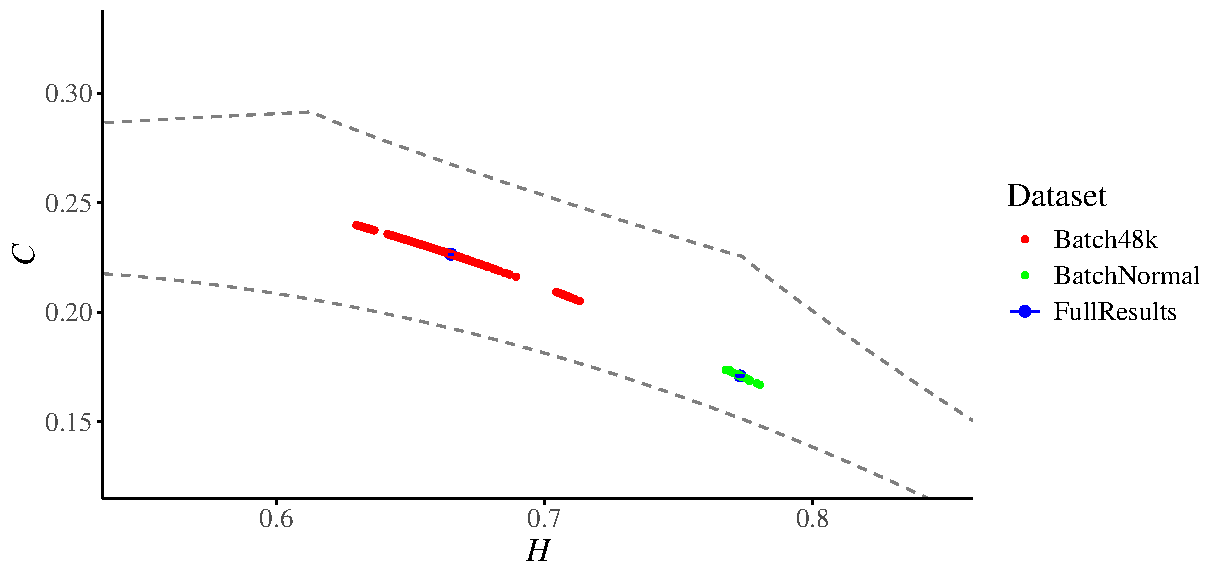
\includegraphics[width=0.8 \textwidth]{confidence_interval}
	\caption{Entropy Complexity Plane}
	\label{fig:EntopyComplexity Plane}
\end{figure}

The general framework for analyzing entropy-complexity planes with confidence intervals are given as follows.
\begin{enumerate}
\item \textbf{Calculate Entropy (H) and Complexity (C):} 
appropriate estimator are Shannon entropy, statistical complexity measures 
\item \textbf{Compute Confidence Intervals:}
Generate multiple resampled datasets to estimate the variance of $H$ and $C$.
\item \textbf{Plot on Entropy-Complexity Plane:}
\begin{itemize}
	\item Axes:x-axis: Entropy $(H)$, y-axis: Statistical complexity $(C)$
	\item Data Points: Plot individual or aggregated results.
	\item Confidence Regions: Represent uncertainty 
\end{itemize}

\item \textbf{Interpretation}
\begin{table}[H]
	\centering
	\begin{tabular}{cr}
		\toprule
		Region of Plane  & Interpretation  \\
		\midrule
		High $H$ and High $C$ & Complex, structured systems \\ 
		Low $H$ and Low $C$ & Simple, predictable systems \\
		High $H$ and Low $C$ & Random/noisy systems \\
		Low $H$ and High $C$ & Non-random systems \\ 
		\bottomrule
	\end{tabular}
	\end{table}

\item \textbf{Statistical testing:}
\begin{itemize}
	\item Compare confidence intervals between groups to assess significant differences.
	\item Overlapping intervals $\rightarrow$ {No significant difference}.
	\item Non-overlapping intervals $\rightarrow$ Potential significance.
\end{itemize}
\end{enumerate}



    



